% !TeX root = ../thuthesis-example.tex

\chapter{服务器端高性能 \emph{insertRecords} 写入机制设计与实现}
经过客户端的预处理与 RPC 层的数据传输,写入请求最终会到达服务器端。服务器端对写入请求进行预处理后,交由存储引擎负责处理写入请求,并将这些数据最终持久化到磁盘上,服务器端的设计与实现对写入性能有至关重要的影响。如 \ref{sec:chap3-sec3-1} 中的实验结果所示,现有 IoTDB 服务器端对写入请求的处理有较大的性能瓶颈,不能满足高并发写入请求的需求。因此,本章将介绍对 \emph{insertRecords} 写入请求所设计的服务器端高性能写入机制。


\section{服务器端 \emph{insertRecords} 写入流程总览}
\ref{sec:chap3-sec2} 节介绍了 IoTDB 服务器端对 \emph{insertRecords} 写入请求执行的总体流程,新的执行流程和原有流程大体相似,单针对之前实验中发现的瓶颈,本工作进行了重新设计以优化写入性能。

\begin{figure}
  \centering
  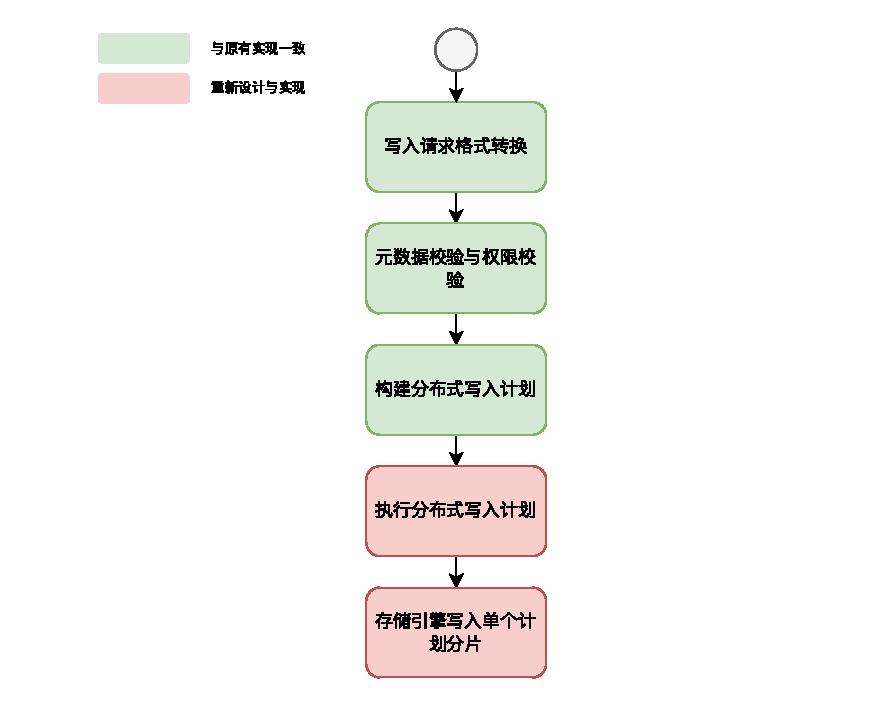
\includegraphics[width=0.9\linewidth]{new-storage-engine.pdf}
  \caption{服务器端 \emph{insertRecords} 写入流程}
  \label{fig:iotdb-insertRecords-flow}
\end{figure}

图 \ref{fig:iotdb-insertRecords-flow} 展示了 \emph{insertRecords} 写入请求到达 IoTDB 服务器端以后的总体执行流程,其中绿色部分代表这些流程与 IoTDB 原有设计基本保持一致,因为它们并不是写入的瓶颈所在;红色部分代表了在原有实现中存在的性能瓶颈,本工作对这些部分进行了重新设计与实现以提高写入性能。


在执行分布式写入计划时,一个写入请求会被分为多个写入计划分片(称为 FragmentInstance,FI),每个分片都是写入到一个 DataRegion 中的计划。根据 DataRegion 的分布,可以将其分为本地 DataRegion 和远程 DataRegion,本地 DataRegion 是指存储引擎所在的节点上的 DataRegion,远程 DataRegion 是指存储引擎所在节点以外的 DataRegion。为了充分利用多核 CPU 的计算能力,本工作将写入本地和写入远程 DataRegion 的过程都设计为了多线程并行执行,以提高写入性能。

在存储引擎写入单个计划分片时,不仅需要将数据记录到内存表中,还需要执行记录写前日志、更新监控信息、维护内存索引等操作。这些操作大部分都不是核心的写入操作,但是却会对写入性能产生较大的影响。因此,本工作通过批量化的形式,将这些操作的代价分摊到多行写入记录上,以减少这些操作对写入性能的影响。例如,原本每写入一行记录就需要记录一次写前日志、更新一次监控信息、维护一次内存索引,现在可以将这些操作批量化,每写入一批记录才执行一次这些操作,这样平均到每一条记录上的代价就大大减小了。最后,为了改善前文提到的使用 \emph{insertRecords} 接口进行写入时写前日志过多的问题,本工作对写前日志进行了压缩,减少了写前日志对磁盘的写入量,提高了写入性能。下面将详细介绍这些优化措施的设计与实现。

\section{多线程并行写入设计与实现}
\subsection{多线程并行写入设计}
图 \ref{fig:fi-parallel-write} 展示了 FragmentInstance 多线程并行写入的总体架构。多线程并行写入的设计分为写入本地 DataRegion 和写入远程 DataRegion 两部分,下面将分别介绍这两部分的设计。

\begin{figure}
  \centering
  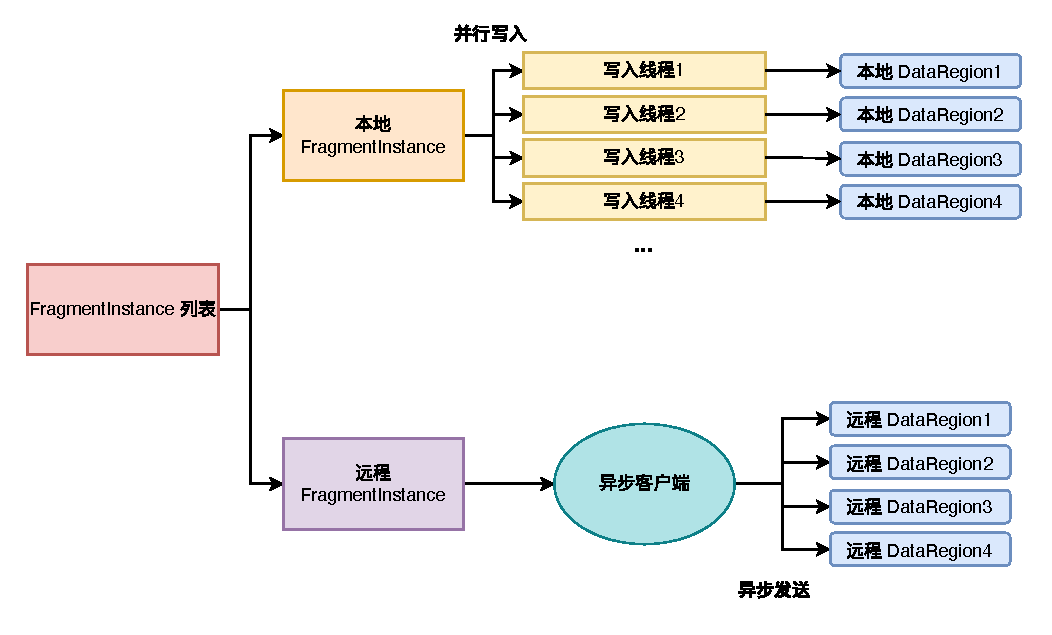
\includegraphics[width=\linewidth]{FragmentInstance写入.pdf}
  \caption{多线程并行写入设计}
  \label{fig:fi-parallel-write}
\end{figure}

在一般的系统中,对一项任务的并行执行通常会构建一个线程池负责此工作,以减少线程创建与销毁的开销,在本工作的设计中遵循了这一种范式。因此,想要实现多线程并行写入,我们首先要确定线程池的大小。如果线程池中的线程数过少,那么无法充分利用多核 CPU 的计算能力,从而无法提高写入性能;如果线程池中的线程数过多,那么会增加线程创建与销毁的开销,反而会降低写入性能。根据线程数与 DataRegion 的个数的比例,可以分为多个线程写一个 DataRegion、一个线程写一个 DataRegion 和一个线程写多个 DataRegion 三种情况。在目前 IoTDB 的设计与实现中,每个 DataRegion 都有一个锁,用于保证对 DataRegion 的读写操作是线程安全的。此外,一个 DataRegion 也对应了一个共识组,共识层为了保证数据的一致性,也持有一个锁。在这样的设计下,针对一个 DataRegion 的写入是串行的,即一次只能有一个线程写入一个 DataRegion。

综合以上因素,本工作选择了一个线程写一个本地 DataRegion 的设计,即每个 DataRegion 都有一个专门的线程负责处理这个 DataRegion 的写入任务。为了处理多个写入请求,每个 DataRegion 的线程都会维护一个写入队列,用于存放待写入的数据。不同写入请求对同一个 DataRegion 的写入任务会被放入同一个队列中,该 DataRegion 对应的写入线程会不断从写入队列中取出任务进行处理。为了避免过多任务堆积,任务队列的大小是有限的,超过了队列的大小后,新的写入请求会被拒绝,并向客户端返回写入失败的信息。写入请求向写入队列提交写入任务后,会获得一个 Future 对象,用于知晓写入任务的执行结果。写入任务执行完成后,Future 对象会被设置为完成状态,并且可以通过 Future 对象获取写入任务的执行结果。

对远程 DataRegion 的写入通过网络发送,在系统内缓存了一个全局的客户端池,它们负责将对远程 DataRegion 写入的 FragmentInstance 异步地发送到对应的节点上,并且返回一个 Future 对象,用于后续的处理。

当写入本地 DataRegion 和远程 DataRegion 的 FragmentInstance 都被异步地分发之后,主写入线程会拿到所有这些 FragmentInstance 对应的 Future 对象,并通过这些对象等待它们全部完成,随后将写入结果返回给客户端。

\subsection{多线程并行写入实现}
为了实现上述的设计,本工作通过一个 FragmentInsertPoolManager 类来管理每个本地 DataRegion 的写入,该类的字段和方法如表 \ref{tabular:fragment-insertion-pool-manager-fields} 和表 \ref{tabular:fragment-insertion-pool-manager-methods} 所示。

\begin{table}
  \centering
  \caption{FragmentInsertPoolManager 类字段}
  \label{tabular:fragment-insertion-pool-manager-fields}
  \begin{tabular}{lp{5cm}p{5cm}}
    \toprule
    字段名 & 字段类型 & 字段描述 \\
    \midrule
    instance & FragmentInsertPoolManager & 单例模式 \\
    executionPoolMap & Map<ConsensusGroupId, ExecutorService> & 记录每个 DataRegion 对应的线程池 \\
    \bottomrule
  \end{tabular}
\end{table}

\begin{table}
  \centering
  \caption{FragmentInsertPoolManager 类方法}
  \label{tabular:fragment-insertion-pool-manager-methods}
  \begin{tabular}{lp{5cm}p{5cm}}
    \toprule
    方法名 & 方法参数 & 方法描述 \\
    \midrule
    getInstance & 无 & 获取 FragmentInsertPoolManager 的单例 \\
    registerPool & 一个 DataRegion 以及一个 ExecutorService & 注册这个 DataRegion 对应的写入线程,便于后续的写入任务分发 \\
    submitTask & ConsensusGroupId 以及写入任务 & 将写入任务提交到对应的 DataRegion 的写入线程池中执行 \\
    \bottomrule
  \end{tabular}
\end{table}

FragmentInsertPoolManager 的核心方法是 registerPool 和 submitTask。当一个 DataRegion 被创建或者恢复时,它会创建一个单线程的线程池,用于执行所有写入到本 DataRegion 的 FragmentInstance,然后调用 FragmentInsertPoolManager 的 registerPool 方法,将这个线程池注册到 FragmentInsertPoolManager 中。当执行写入请求的主线程开始执行分布式写入计划时,它会调用 FragmentInsertPoolManager 的 submitTask 方法,将写入任务提交到对应的 DataRegion 的写入线程池中执行。

对于远程的 DataRegion 写入,本工作通过网络的异步发送来完成并行写入。在 IoTDB 中,每个 DataNode 都为与其他 DataNode 的连接维护了一个全局的客户端池。当需要写入远程 DataRegion 时,主写入线程会从客户端池中获取一个客户端,然后将写入任务通过客户端的异步发送接口发送到对应的 DataNode 上。异步发送接口由 Thrift 实现,这个接口要求上层传入一个回调函数,当发送完成后会调用这个回调函数。主写入线程通过这个回调函数来知晓写入任务的执行结果。

由于网络传输的原因,写入远端 DataRegion 的耗时会更久。为了更高效地执行写入,主写入线程会先发送对远端 DataRegion 的写入请求,然后再将对本地 DataRegion 的写入请求提交到线程池中执行,此时远端和本地的写入都在并行执行。等到所有的写入请求都执行完成后,主写入线程再将写入结果返回给客户端。

\section{批量化写入设计与实现}
\subsection{批量化写入设计}
批量化写入一共分为三点:批量化写前日志、批量化更新监控信息和批量化维护内存索引。在 IoTDB 的设计中,每次写入一行数据都会记录一次写前日志、更新一次监控信息和维护一次内存索引,这些操作都会对写入性能产生较大的影响。因此,本工作将这些操作批量化,每次写入一批数据才执行一次这些操作,以减少这些操作对写入性能的影响。

\subsubsection{批量化写前日志}
\begin{figure}
  \centering
  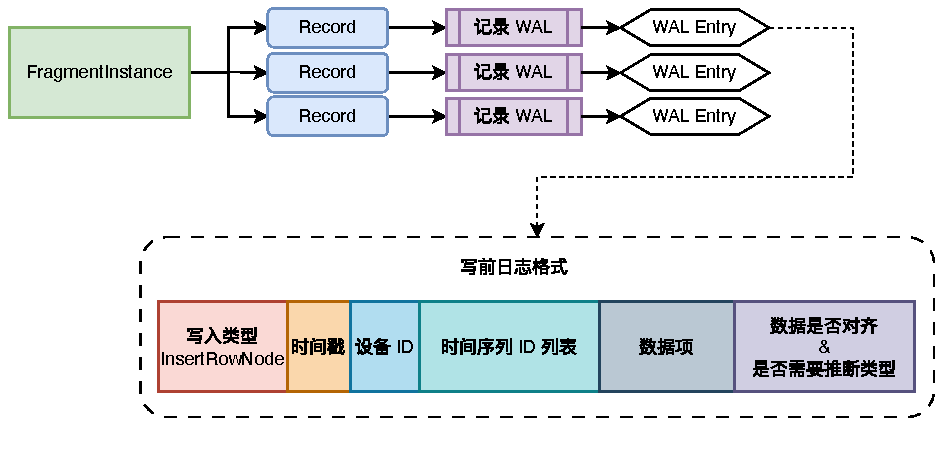
\includegraphics[width=\linewidth]{origin-wal-format.pdf}
  \caption{原有写入日志格式}
  \label{fig:origin-wal-format}
\end{figure}

图 \ref{fig:origin-wal-format} 展示了在原有 IoTDB 的实现中,一个 FragmentInstance 在写入时记录写前日志的流程和格式。对一个 FragmentInstance 中的每一行记录,都需要单独记录一次写前日志,每次都需要重复记录这些记录的时间戳、设备 ID、时间序列 ID 和数值项等,而这其中有相当一部分信息是重复的。这样的设计会导致写前日志的体积过大,对磁盘的写入量也会增加,从而影响写入性能。

// TODO:判断是否要写写前日志批量化的工作
\subsubsection{批量化更新监控信息}
 IoTDB 的监控系统负责监控 IoTDB 运行时的各类指标,以便于用户和开发者了解 IoTDB 的状态,并进行运维和调优。
 在 IoTDB 现有的实现中,每写入一个 FragmentInstance 中的一行记录,就需要更新对应的监控信息,包括创建内存表的耗时、写入写前日志的耗时、写入内存表的耗时、更新内存缓存的耗时等。监控系统为这些监控项都维护了对应的直方图,因此每次写入一行记录需要更多这些监控项对应的直方图。从 \ref{sec:chap3-sec3-1} 节中对 \emph{insertRecords} 和 \emph{insertTablets} 的实验中可以看出,\emph{insertRecords} 写入时更新监控信息的开销明显较大。因此,本工作将这些监控信息的更新批量化,每次写入一批数据才更新一次这些监控信息,以减少这些操作对写入性能的影响。

 为了实现这一点,我们修改了更新监控信息的时机和逻辑。每行记录在写入时,仍会记录各个阶段的耗时,但不会将这些耗时立马更新到监控系统里,而是将这些耗时记录在一个本地的数据结构中。这个数据结构只记录这一个写入请求的监控指标,当这个写入请求的每一个 FragmentInstance 都写完了以后,再统一将这些监控指标更新到监控系统中。在这样的设计下,原本执行一次 \emph{insertRecords} 更新监控框架的次数为写入数据的行数,现在则变成了一次,这样就大大减少了更新监控信息对写入性能的影响。

\subsubsection{批量化维护内存缓存}
IoTDB 支持一种名为 Last 查询的查询方式,它可以查询某个时间序列写入数据库的最后一个数据点。为了提高 Last 查询的性能,IoTDB 在内存中维护了一个名为 LastCache 的缓存,其中保存了每个时间序列写入数据库的最后一个数据点。在每次写入时,都需要对这个缓存进行维护。在 IoTDB 的现有实现中,每次写入一行记录都要维护一次这个缓存,这样会导致写入性能下降,从表 \ref{tabular:insert-records-profile-result} 中可以看出,维护内存缓存在 \emph{insertRecords} 写入的性能开销中占有较大的比例。

为了减少维护内存缓存对写入性能的影响,本工作将维护内存缓存的操作批量化,每次写入一个 FragmentInstance 之后才批量化地更新一次缓存。并且,更新缓存之前,先对 FragmentInstance 中的数据进行排序和去重,只更新写入的时间序列的最后一个点。之所以这样设计,是因为 LastCache 的设计比较复杂,反复更新 LastCache 的代价较大,因此我们选择提前处理好数据,以尽可能地减少对 LastCache 的更新。
\subsubsection{批量化写入内存表}
在如今的 \emph{insertRecords} 实现中,写入内存表的操作是行式的,即数据是一行一行地写入到内存表中的。这样的效率并不高,因为每写入一行都要调用许多辅助函数,函数调用的开销无法均摊。此外,这样的写入方式对 CPU 的缓存也并不友好\cite{boncz2005monetdb}。为了提高写入内存表时的效率,本工作将这个过程批量化,在写入之前先对数据进行排序和归类,将写入到同一个内存表的数据聚集到一起,然后一次性地写入到内存表中,以减少函数调用的开销和提高 CPU 缓存的命中率。

\subsection{批量化写入实现}
本工作对上述批量化执行设计进行了实现。

\section{写前日志压缩设计与实现}
\subsection{写前日志压缩设计}
\subsection{写前日志压缩实现}